\chapter{Que sait-on sur le modèle compressible ?}
\renewcommand\partie{\Partie\ Chapitre \thechapter}
\label{ch-12}

%\medskip
\minitoc  

\bigskip

Lorsque la contrainte d'incompressibilité qui servait de fermeture au système d'équation est relaxée, le modèle n'est plus fermé. Dans ce chapitre, seront définis différents types de fermeture en considérant toujours une pression isotrope. On regardera ce qu'il advient du taux de cascade dans le chapitre suivant.   

\section{Energétique du modèle \acs{MHD} non fermé}
\label{sec-121}
Si l'on reprend les équations du modèle \acs{MHD}, dérivées du modèle cinétique (voir synthèse \ref{synt-02}), et que l'on suppose une pression isotrope, on obtient le système suivant, écrit avec la vitesse d'Alfvén $\boldsymbol{v_A}=\frac{\boldsymbol{B}}{\sqrt{\mu_0\rho}}$, : 
\begin{eqnarray}
\partial_t \rho + \nabla \cdot \left(\rho \boldsymbol{v}\right) &=& 0 \label{eq:model_cpi_r}, \\
\partial_t \left(\rho \boldsymbol{v}\right) + \nabla \cdot \left(\rho \boldsymbol{v}\boldsymbol{v} - \rho \boldsymbol{v_A}\boldsymbol{v_A}\right) +  \nabla p_*  &=& 0 \label{eq:model_cpi_v}, \\
3 \partial_t p + \nabla \cdot \left( 3 p\boldsymbol{v} + 2\boldsymbol{q}\right) + 2 p \nabla \cdot \boldsymbol{v} & =& 0 \label{eq:model_cpi_p}, \\
\partial_t \boldsymbol{v_A} -  \nabla \cdot \left(\boldsymbol{v_A}\boldsymbol{v} - \boldsymbol{v}\boldsymbol{v_A}\right) +  \boldsymbol{v}  \nabla \cdot \boldsymbol{v_A} -  \frac{\boldsymbol{v_A}}{2}  \nabla \cdot \boldsymbol{v} &=& 0 .\label{eq:model_cpi_b}
\end{eqnarray}
La contrainte sur le champ magnétique, $\nabla \cdot \boldsymbol{B}=0$, peut s'écrire : $\nabla \cdot \left(\rho \boldsymbol{v_A}\right) = - \rho \nabla \cdot \boldsymbol{v_A} $.
Ce système n'est pas fermé, mais avant de le fermer, regardons ce qu'il nous indique en termes d'énergétique.  
L'équation de densité d'énergie cinétique $E_c = \frac{1}{2}\rho \boldsymbol{v}^2$ obtenue via \eqref{eq:model_cpi_r} et \eqref{eq:model_cpi_v} est :
\begin{equation}
 \label{eq:model_cpi_k}   \partial_t E_c +\nabla \cdot \left(E_c \boldsymbol{v} + p_* \boldsymbol{v}- \rho \boldsymbol{v} \cdot \boldsymbol{v_A}\boldsymbol{v_A}\right)   = -  \rho \boldsymbol{v_A}  \boldsymbol{v_A} : \nabla \boldsymbol{v} + p_* \nabla \cdot \boldsymbol{v}.
\end{equation}
L'équation de densité d'énergie magnétique $E_m = \frac{1}{2}\rho \boldsymbol{v_A}^2$ obtenue via \eqref{eq:model_cpi_r} et \eqref{eq:model_cpi_b} est :
\begin{equation}
  \label{eq:model_cpi_m}   \partial_t E_m  +\nabla   \cdot  \left(E_m\boldsymbol{v}\right)  = \rho  \boldsymbol{v_A}\boldsymbol{v_A}  : \nabla \boldsymbol{v}- p_m  \nabla \cdot \boldsymbol{v}.
\end{equation}
On remarque que l'échange entre ces deux canaux énergétiques se fait à travers la pression magnétique et un terme croisé (termes de droite de \eqref{eq:model_cpi_m}) similaire au cas incompressible. La densité d'énergie totale moyenne $\left<E_{tot}\right> = \left< E_c + E_m + E_u\right>$ étant un invariant du système, cela nous autorise, a priori, à appliquer la méthode résumée dans la section \ref{synt-11} pour en étudier la cascade. Afin que cette énergie soit conservée, il faut ajouter une équation annulant le terme source dépendant de $p$ dans l'équation d'énergie cinétique \eqref{eq:model_cpi_k}. Cette équation est l'équation de densité d'énergie interne, $E_u = \rho u$ avec $u$ l'énergie interne spécifique, dans laquelle on doit aussi faire figurer un terme de flux de chaleur, $\nabla \cdot \boldsymbol{q}$, :
\begin{equation}
   \label{eq:model_cpi_u}  \partial_t E_u +\nabla \cdot \left(E_u \boldsymbol{v} + \boldsymbol{q}\right)   = - p \nabla \cdot \boldsymbol{v}.
\end{equation}
L'équation de densité d'énergie totale, $E_{tot} = E_c + E_m + E_u$, est alors : 
\begin{equation}
   \label{eq:model_cpi_e}  \partial_t E_{tot} +\nabla \cdot \left(E_{tot} \boldsymbol{v} + p_* \boldsymbol{v}- \rho \boldsymbol{v} \cdot \boldsymbol{v_A}\boldsymbol{v_A} + \boldsymbol{q}\right)   = 0.
\end{equation}
On peut remarquer que dans le cas incompressible, l'énergie interne \eqref{eq:model_cpi_u} est découplée de l'énergie cinétique \eqref{eq:model_cpi_k} et par ce biais de l'énergie magnétique \eqref{eq:model_cpi_m} puisque $p \nabla \cdot \boldsymbol{v} = 0$. Via cette méthode basée sur un bilan, nous obtenons, indépendamment de la fermeture, une équation d'évolution pour l'énergie interne [\cite{eckart_thermodynamics_1940}]. L'obtention d'une équation de densité d'énergie totale est donc possible sans expliciter de fermeture qui pourra être fixée dans un second temps. On qualifiera de générales, les équations \eqref{eq:model_cpi_u} et \eqref{eq:model_cpi_e} applicables à toutes données, tous modèles respectant le comportement des moments fluides $\rho$ \eqref{eq:model_cpi_r} et $\boldsymbol{v}$ \eqref{eq:model_cpi_v} obtenus via l'équation de Vlasov et l'équation d'induction \eqref{eq:model_cpi_b}. Mais cette description n'est pas complète, pas fermée, puisque rien n'y impose le respect de l'équation \eqref{eq:model_cpi_p} concernant $p$ qui pourrait être définie autrement, et $\boldsymbol{q}$ reste indéfini. Cette observation présage la possibilité d'obtenir une loi exacte tout aussi générale sur la cascade de densité d'énergie totale comme on le verra dans le Chapitre \ref{ch-13}. 

\section{Fermetures thermodynamiques}
\label{sec-122}
En MHD compressible avec pression isotrope, l'équation de fermeture est souvent une relation entre la pression, $p$, et la densité, $\rho$, issue de la thermodynamique et venant se substituer à l'équation sur la pression \eqref{eq:model_cpi_p}\footnote{On pourrait aussi fermer au niveau des moments suivant via une loi de Fourier sur le flux de chaleur, $\boldsymbol{q} = - \kappa \nabla T$ [\cite{belmont_introduction_2018}], ou la fermeture à l'ordre 4 proposé par \cite{chust_closure_2006} par exemple. On ne détaillera pas ces possibilités ici mais on notera que le flux de chaleur peut, via $\kappa$, la viscosité thermique, n'avoir un impact qu'aux petites échelles, similairement aux dissipations visqueuse et résistive [\cite{eyink_cascades_2018}].}. Par la suite, on appellera thermodynamique tout ce qui est relatif à la densité, la pression, l'énergie interne, etc. (grandeurs supposément définies et convergentes dans le cadre fluide) et pouvant relever du champ de discipline empirique de la thermodynamique à l'équilibre [\cite{borel_thermodynamique_2005}]  possiblement étendu au cadre hors équilibre [\cite{livadiotis_non-equilibrium_2012}].

Le premier principe de la thermodynamique peut s'écrire 
\begin{equation}
\label{eq:thermo_L1} du =  \dj \mathcal{Q} + \dj \mathcal{W} = Tds + \frac{p}{\rho^2} d\rho,
\end{equation}
avec $\mathcal{Q}$ la chaleur et $\mathcal{W}$ le travail de pression, $\dj$ correspond à l'élément de calcul différentiel inexact et $d$ à l'élément exact. L'élément inexact signifie que le résultat d'une intégration sera chemin-dépendant (pour plus d'information se référer à \cite{borel_thermodynamique_2005}). L'élément différentiel exact peut servir à créer une dérivée totale ou partielle. En construisant la dérivée temporelle totale, qui s'écrit en fonction des dérivées partielles $d_t = \partial_t + \boldsymbol{v} \cdot \nabla $, et en injectant l'équation de densité de masse \eqref{eq:model_cpi_r}, on trouve, à partir de \eqref{eq:thermo_L1}, une équation sur la densité d'énergie interne : 
\begin{equation}
\label{eq:thermo_u}   d_t \left(\rho u\right) = \rho T d_t s - \left(p+\rho u\right)\nabla \cdot \boldsymbol{v}.
\end{equation}
Cette équation est compatible avec l'équation \eqref{eq:model_cpi_u} si $\nabla \cdot \mathbf{q} = - \rho T d_t s$, $s$ étant l'entropie spécifique et $T$ la température. Ces équations sont compatibles avec l'équation de pression \eqref{eq:model_cpi_p} si l'on impose $\rho u = \frac{3}{2} p$. On verra que ce n'est pas forcément le cas avec les fermetures de type thermodynamique. 

Dans le cadre thermodynamique original [\cite{borel_thermodynamique_2005}], la définition des dénominations <<polytrope>>, <<isochore>>, <<isobare>>, <<isotherme>> ou <<isentrope>> ne s’applique qu’à des transformations : 
\begin{itemize}
    \item isochore (ou incompressible puisque $\rho = m/V$) signifie à volume $V$ constant
    \item isobare signifie à pression $p$ constante,
    \item isotherme signifie à température $T$ constante, 
    \item isentrope signifie à entropie $s$ constante, elle ne peut être ni créée ni échangée par transfert thermique, 
    \item adiabatique signifie sans transfert thermique $\dj \mathcal{Q}$, c'est-à-dire sans échange d'entropie (equivalente à l'isentrope dans le cas réversible où aucune entropie n'est crée),
    \item polytrope signifie à $\sigma = \frac{Tds}{Vdp}$, le facteur polytrope, constant.
\end{itemize}
Alors qu'en astrophysique et physique des plasmas, on entend ces termes en tant que noms de fermeture caractérisant le système. Ici, dans une volonté de clarifier cet usage, on considérera qu’un système décrit idéalement avec l’une de ces caractéristiques est un système dans lequel la quantité caractérisée ne pourra évoluer qu’en suivant le type de transformation associée. En réalité, ces caractéristiques coexistent souvent, l'une pouvant dominer les autres, par exemple dans les plasmas spatiaux d'après \cite{livadiotis_non-equilibrium_2012}. 

L'hypothèse polytrope apparaît plus générale dans le sens où, suivant la valeur de $\sigma$, on peut se retrouver dans le cadre des hypothèses isochore, isobare, isotherme, adiabatique ou isentrope [\cite{borel_thermodynamique_2005}]. D'après \cite{horedt_polytropes_2004}, cette hypothèse a été introduite par \cite{chandrasekhar_introduction_1939} en astrophysique via la définition : $pV^{\gamma}$ constant avec $\gamma = \frac{c_p - c}{c_V - c}$, nommé indice spectral ou indice polytropique. $c$ est, ici, $\frac{d\mathcal{Q}}{dT}$ la chaleur spécifique, $c_p$ la chaleur spécifique à pression constante et $c_V$ celle à volume constant. Cette définition rappelle celle de l'indice adiabatique $\gamma_a = c_p/c_V$. On peut d'ailleurs réécrire $\gamma$ en fonction de $\gamma_a$ en se plaçant dans le cadre d'un gaz parfait ($pV \propto T$) et en utilisant les relations (1.2.19) à (1.2.24) de \cite{horedt_polytropes_2004}. Ainsi $\gamma = \left(\gamma_a - 1\right) K + \gamma_a$ avec $K = \frac{\dj  \mathcal{Q}}{\dj \mathcal{W}} = \frac{Tds}{-pdV}$. Sachant que $d\left(pV^{\gamma}\right) = 0$, le lien entre $pV^{\gamma}$ et $\sigma = \frac{Tds}{Vdp}$ est $\sigma = K/\gamma = \frac{1-\gamma_a/\gamma}{\gamma_a-1}$. D'où l'équivalence des définitions\footnote{L'intérêt de la définition via $\sigma$ met en lumière la différence entre les transformations polytropes et adiabatique/isentrope ($\sigma = 0 $ et $\gamma = \gamma_a$) qui semblent souvent confondues en astrophysique [\cite{eyink_cascades_2018}], peut-être car le flux de chaleur semble \og disparaître \fg{} dans l'obtention de la forme explicite de l'énergie interne.} via $\sigma$ et $\gamma$. 

La \figref{fig:schema_thermo} inspirée de \cite{livadiotis_non-equilibrium_2012}, complétée avec les valeurs de $\sigma$ et quelques exemples de plasmas spatiaux données par \cite{livadiotis_long-term_2018}, résume le lien entre les différentes fermetures et l'hypothèse polytrope. Les plasmas spatiaux pouvant être modélisés comme des gaz parfaits monoatomiques, $\gamma_a = 5/3$ et dans le cas isochore, $\sigma = \frac{1}{\gamma_a-1}=3/2$.
\begin{figure}[!ht]
 \centering
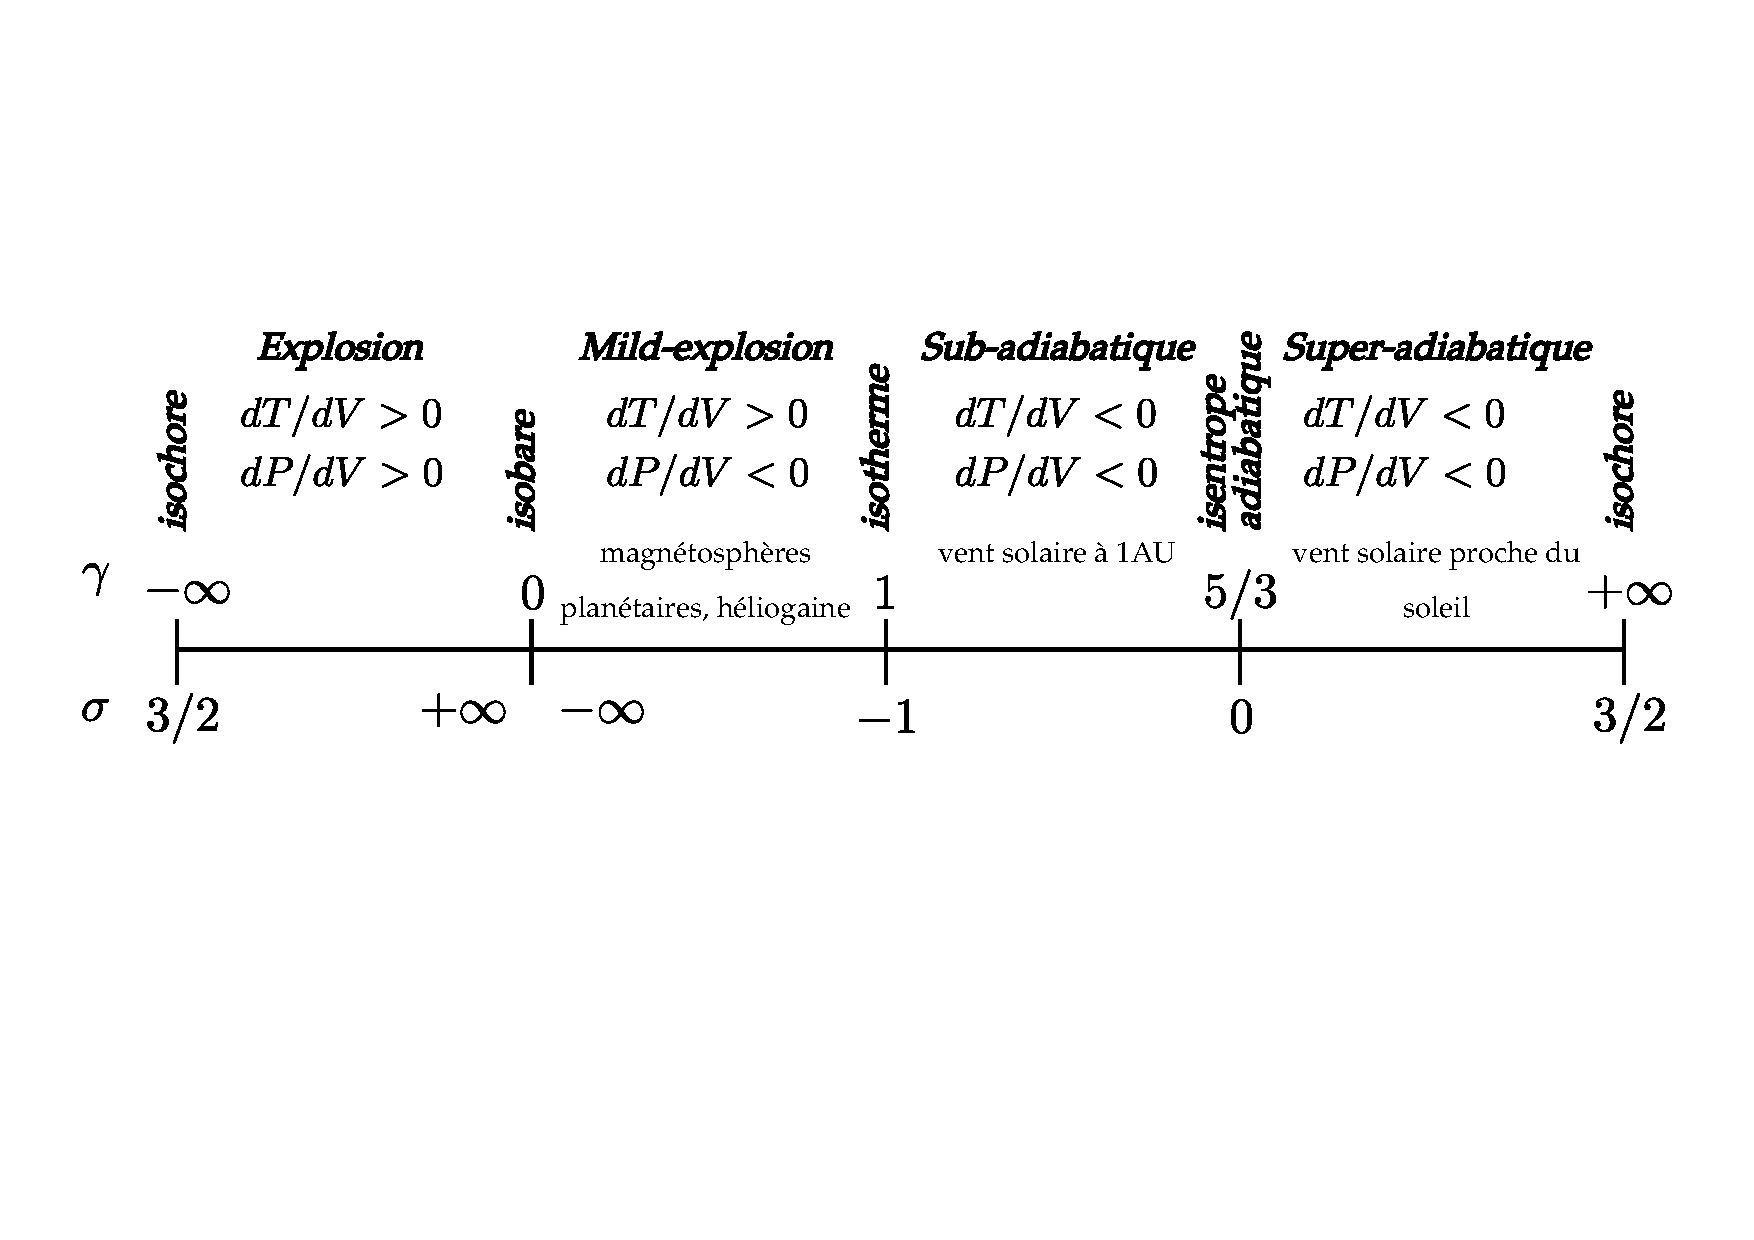
\includegraphics[width=0.9\linewidth,trim=1cm 8cm 1cm 5.5cm, clip=true]{./Part_1/images/schema_thermo.pdf}
\caption{Transformations thermodynamiques et intervalles en fonction du $\gamma$ du milieu [\cite{livadiotis_non-equilibrium_2012}] et du $\sigma$ [\cite{borel_thermodynamique_2005}], exemple de plasmas spatiaux [\cite{livadiotis_long-term_2018}]. Adiabatique et isentrope y sont confondues dans le cas réversible.}
\label{fig:schema_thermo}
\end{figure}

Dans le premier principe \eqref{eq:thermo_L1} et l'équation d'énergie interne \eqref{eq:thermo_u}, l'utilisation de $\sigma$ permet d'écrire : 
\begin{eqnarray}
\label{eq:thermo_sig_L1}    du &=& \dj \mathcal{Q} + \dj \mathcal{W} = \left(K+1\right) \dj \mathcal{W} = \left(\sigma \gamma + 1\right) \dj \mathcal{W} ,\\
\label{eq:thermo_sig_u}    d_t\left(\rho u\right) &=& -\left[\left(\sigma \gamma + 1\right) p + \rho u\right] \nabla \cdot \boldsymbol{v} ,\\
 \label{eq:thermo_sig_q}   &\Rightarrow& \nabla \cdot \boldsymbol{q} = -\rho T d_t s = \sigma \gamma p \nabla \cdot \boldsymbol{v}.
\end{eqnarray}
D'un autre côté, la relation entre $p$ et $V$ peut s'écrire $p \propto \rho^{\gamma}$. Cela donne l'équation : 
\begin{eqnarray}
 \label{eq:thermo_sig_p}   d_t p &=& -\gamma p \nabla \cdot \boldsymbol{v}.
\end{eqnarray}
Cette équation est compatible avec l'équation de pression du modèle fluide \eqref{eq:model_cpi_p} si :
\begin{eqnarray}
\label{eq:thermo_sig_gq}     \left(\frac{5}{3} -\gamma\right) p \nabla \cdot \boldsymbol{v} = -\frac{2}{3} \nabla \cdot \boldsymbol{q} 
\label{eq:thermo_sig_g}     &\Rightarrow& \left(\frac{5}{3} +\left(\frac{2}{3}\sigma-1\right)\gamma\right) p \nabla \cdot \boldsymbol{v} = 0 .
\end{eqnarray}
Par ces relations, on remarque que l'hypothèse polytrope peut nous permettre de fermer le modèle fluide au niveau du troisième moment $\boldsymbol{q}$ en injectant \eqref{eq:thermo_sig_q} dans l'équation de $p$ \eqref{eq:model_cpi_p}, ou au niveau du deuxième, $p$, en utilisant $\gamma$ et en injectant $p \propto \rho^{\gamma}$ dans \eqref{eq:model_cpi_v}\footnote{Usuellement, comme on cherche à fermer le modèle aussi tôt que possible, on ferme au niveau du deuxième moment. L'information sur le flux de chaleur est alors perdue d'où la confusion entre isentrope et polytrope.}. L'hypothèse adiabatique, isentrope si réversible, $\gamma=\gamma_a$ et $\nabla \cdot \boldsymbol{q}=0$, est retrouvée dans l'évolution fluide de $p$ si l'on se place dans le cadre d'un gaz parfait monoatomique $\gamma_a = 5/3$ d'après \eqref{eq:thermo_sig_gq}. Dans le cas isotherme, on retrouve dans \eqref{eq:thermo_sig_gq} ou \eqref{eq:thermo_sig_L1}, $\dj \mathcal{W} = - \dj \mathcal{Q}$, c'est-à-dire $du = 0$. En effet, la variation d'énergie interne d'un gaz parfait ne dépendant que de la température, ne peut qu'être nulle sous l'hypothèse d'isothermie. Les cas isochore (ou incompressible) et isobare sont plus délicats. Dans le cas isochore, le produit $\gamma \nabla \cdot \boldsymbol{v}$ qui apparaît dans toutes les expressions de \eqref{eq:thermo_sig_L1} à \eqref{eq:thermo_sig_g}, tend vers $\infty \times 0$. Dans le cas isobare, $\infty \times 0$ apparaît dès que $\sigma \gamma$ est présent dans l'équation. Ces limites du cas polytrope sont donc problématiques dans la définition de $u$. Elles doivent être traitées indépendamment. Dans le cas isochore, $\dj \mathcal{W} = 0$ et l'énergie interne vérifie $d_t u + \nabla \cdot \boldsymbol{q} = 0 $. L'hypothèse isobare, quant à elle, ferme le système fluide au niveau de l'équation \eqref{eq:model_cpi_v}. L'équation d'énergie interne est alors  $\partial_t u + \nabla \cdot \left(u \boldsymbol{v} + \boldsymbol{q} + p_0 \boldsymbol{v}\right) = 0 $. Pour ces deux fermetures, l'énergie interne est conservée et n'échange plus avec les énergies cinétique et magnétique \footnote{La cascade d'énergie cinétique et magnétique peut alors être traitée indépendamment de celle d'énergie interne.  Cela a été fait dans le Chapitre \ref{ch-11} dans le cadre incompressible.}.

Dans le cadre de la fermeture polytrope, on peut écrire $p = \frac{c_s^2}{\gamma} \rho$, avec $c^2_s = \frac{\partial p}{\partial \rho} \propto \rho^{\gamma-1}$ le carré de la vitesse thermique. Pour ce qui est de la variation d'énergie interne spécifique, elle devient :
\begin{eqnarray}
\label{eq:thermo_pol_du} d u &=& \left(\sigma \gamma+1\right) \frac{p}{\rho^2} d \rho =  \left(\sigma \gamma+1\right) \frac{p}{\rho^{\gamma}} \rho^{\gamma -2} d \rho \\
&=& \left\{ \begin{array}{lcl} \frac{\sigma \gamma+1}{\gamma-1} \frac{p}{\rho^{\gamma}} d\left( \rho^{\gamma-1} \right)  &\textrm{ si }&  \gamma \neq 1\\
\left(\sigma+1\right) \frac{p}{\rho} d \left(\ln{\rho}\right)  &\textrm{ si }&  \gamma = 1
\end{array} \right. .
\end{eqnarray}
Et par intégration :
\begin{eqnarray}
\label{eq:thermo_pol_u} u - u_I &=& \left\{ \begin{array}{lclcl} \frac{\sigma \gamma+1 }{\gamma-1} \frac{p}{\rho^{\gamma}} \left(\rho^{\gamma-1} - \rho_I^{\gamma-1}\right) &=& \frac{\sigma \gamma+1 }{\gamma-1} \frac{c_s^2}{\gamma} \left(1 - \left(\frac{\rho_I}{\rho}\right)^{\gamma-1}\right)  & \textrm{ si } & \gamma \neq 1\\
   \left(\sigma+1\right) \frac{p}{\rho} \ln \frac{\rho}{\rho_I} &=& \left(\sigma+1\right) c_s^2 \ln \frac{\rho}{\rho_I} &\textrm{ si }&  \gamma = 1 
   \end{array} \right. ,
\end{eqnarray} 
en notant $u_I$ et $\rho_I$ les constantes d'intégrations.
Dans le cas particulier de la fermeture isotherme, $\gamma = 1$, $\sigma = -1$, $p = c^2_s \rho$ avec $c_s$ constante et $du = 0$. 

\section{Thermodynamique et turbulence} \label{sec-112bis}

La cascade turbulente pourrait être, dans les plasmas spatiaux peu collisionnels, une réponse au problème du chauffage. En définissant le chauffage comme la variation de température et sachant que pour un gaz parfait, l'énergie interne ne dépend que de la température\footnote{Dans un gaz parfait, on suppose que les particules n'interagissent pas entre elles. Donc qu'elles soient éloignées ou proches n'influera pas sur leur énergie individuelle. Par conséquent, l'énergie interne est indépendante de la densité. Cependant, la densité d'énergie interne dépendra de $\rho$ et $T$.}, il est facile de définir le chauffage comme tout transfert d'énergie vers l'énergie interne, appelée aussi énergie thermique [\cite{cassak_pressure-strain_2022}]. Le terme de pression dans l'équation \eqref{eq:model_cpi_v} s'interprète alors comme les termes visqueux et résistifs abordés dans le Chapitre \ref{ch-11}, c'est-à-dire comme un terme \og dissipatif\fg{}. Mais, ce serait oublier que la cascade turbulente permet de faire le lien entre les grandes échelles, \acs{MHD}, où la validité de l'hypothèse de gaz parfait est cohérente puisque l'on néglige les interactions entre ions et électrons, et les petites échelles, cinétiques, où les interactions commencent à apparaître à travers le champ électromagnétique. Il manque donc un ingrédient à la définition du chauffage comme un transfert d'énergie vers l'énergie interne. Si l'on regarde la dissipation visqueuse ou résistive, elle vient réduire l'énergie du système, mais elle apparaît aussi dans l'équation d'entropie [\cite{eyink_cascades_2018}]. Chauffer ainsi va donc venir augmenter l'entropie du plasma. {\bf La définition du chauffage adaptée à l'étude de la turbulence est donc celle d'un transfert énergétique avec l'énergie interne impactant l'entropie. Le taux de cascade doit donc prendre en compte l'énergie étant transférée isentropiquement à l'énergie interne.}

Cette définition du chauffage justifie l'hypothèse proposée par \cite{galtier_exact_2011} que seul le terme de travail $\dj \mathcal{W}$ de l'énergie interne affecte la cascade dans la zone inertielle. Cette hypothèse revient à supposer une zone inertielle isentrope telle que $\sigma = 0$. Si le système global est fermé tel que $\gamma \neq \gamma_a$, le terme de chaleur $\dj \mathcal{Q}$ jouera un rôle aux autres échelles afin que les relations thermodynamiques soient respectées dans le système global. La fermeture considérée par \cite{galtier_exact_2011} est la fermeture isotherme qui dans l'hypothèse d'une zone inertielle isentrope implique :  $\gamma = 1$, $\sigma = 0$, $p = c^2_s \rho$ avec $c_s$ constante et $du = \dj \mathcal{W} \Rightarrow u-u_I = \frac{p}{\rho} \ln \frac{\rho}{\rho_I} $. On appellera cette fermeture, qui n'est valable que dans la zone inertielle, <<isentrope-isotherme>> afin d'expliciter la nuance existant entre l'isotherme basique tel que $du = 0$ et l'isotherme étudié dans le cadre d'une cascade isentrope. En suivant cette logique, je me suis intéressée dans \cite{simon_general_2021} à la fermeture <<isentrope-polytrope>> telle que $\sigma = 0$,  $p = \frac{c_s^2}{\gamma} \rho^{\gamma}$ et 
\begin{eqnarray}
\label{eq:thermo_ipol_u} u - u_I &=& \left\{ \begin{array}{lclcl} \frac{1 }{\gamma-1} \frac{p}{\rho^{\gamma}} \left(\rho^{\gamma-1} - \rho_I^{\gamma-1}\right) &=& \frac{+1 }{\gamma-1} \frac{c_s^2}{\gamma} \left(1 - \left(\frac{\rho_I}{\rho}\right)^{\gamma-1}\right)  & \textrm{ si } & \gamma \neq 1\\
    \frac{p}{\rho} \ln \frac{\rho}{\rho_I} &=&  c_s^2 \ln \frac{\rho}{\rho_I} &\textrm{ si }&  \gamma = 1 
   \end{array} \right. .
\end{eqnarray} 
Dans l'usage des formes explicites de l'énergie interne dans les calculs de lois exactes avec l'hypothèse polytrope, les constantes sont souvent annulées entre elles. Par exemple, dans le cas <<isentrope-polytrope>>, \cite{banerjee_kolmogorov-like_2014} considère comme forme explicite de l'énergie interne $ \rho u = \frac{1}{\left(\gamma-1\right)} p $. Contrairement à ce travail, nous avons choisi de maintenir une forme de compatibilité avec la fermeture <<isentrope-isotherme>> de \cite{galtier_exact_2011} (si $u = u_I$ alors $u = 0$) dans nos choix de constantes.

Sont résumés dans la \tabref{tab:fermetures}, les caractéristiques, dénominations et choix de constante des fermetures définies polytropiquement via $\sigma$ et $\gamma$ qui serviront par la suite. 
\begin{table}[!ht]
\begin{center}
\begin{tabular}{ c|c|c } 
Nom & Paramètres & Energie interne explicite\\
\hline
Polytrope (hors isotherme)  & $\{\sigma,\gamma \neq 1 \}$  & $ \frac{\sigma \gamma+1 }{\gamma-1} \frac{p}{\rho^{\gamma}} \left(\rho^{\gamma-1} - \rho_I^{\gamma-1}\right) $    \\
Isotherme  & $\{-1,1\}$ & $  u = 0$     \\
Isentrope-polytrope (hors isotherme) & $\{0,\gamma \neq 1\}$ & $ \frac{1 }{\gamma-1} \frac{p}{\rho^{\gamma}} \left(\rho^{\gamma-1} - \rho_I^{\gamma-1}\right)  $  \\
Isentrope-isotherme & $\{0,1\}$  & $ u = \frac{p}{\rho} \ln \frac{\rho}{\rho_I}$  \\
\end{tabular}
\end{center}
\caption{Fermetures et relations associées. La forme de l'énergie interne de l'isentrope-isotherme est calquée sur celle utilisée par \cite{galtier_exact_2011}. Les autres sont définies de telle sorte à maintenir une forme de compatibilité : si $u = u_I$ alors $u = 0$. Celle de l'isentrope-polytrope est donc légèrement différente de celle utilisée par \cite{banerjee_kolmogorov-like_2014}. $\frac{p}{\rho}$ peut aussi s'écrire $\frac{c_s^2}{\gamma}$ et $p \propto \rho^{\gamma}$. \label{tab:fermetures}}
\end{table}

\cite{aluie_conservative_2012} observent en détail la cascade d'énergie cinétique et magnétique dans différentes simulations subsoniques à transoniques. Le transfert cinétique-interne via la pression semble n'avoir lieu qu'à grande échelle dans une zone qu'ils appellent <<zone de conversion>>, à plus petites échelles cette contribution reste constante. Ils en déduisent un découplage des cascades d'énergie cinétique et d'énergie interne et l'existence d'une zone inertielle cinétique. \cite{eyink_cascades_2018} déduisent aussi, analytiquement, un effet à grande échelle de la pression qui permettrait d'alimenter des structures cohérentes et de réduire l'entropie à grande échelle. Cela induirait une cascade inverse d'entropie vers les grandes échelles et un équilibre s'établirait entre les cascades d'énergie totale et d'entropie. Aucun de ces résultats ne prouve que l'énergie interne ne cascade pas. Ne pas la prendre en compte dans l'estimation du taux de chauffage comme le propose \cite{hellinger_von_2018} est donc hasardeux et n'est justifiable que dans le cas subsonique où sa contribution semble mineure [\cite{andres_energy_2018,ferrand_compressible_2020}] ou à des échelles plus faibles que celle où l'impact de la pression semble majeur [\cite{aluie_conservative_2012}]. Etudier la cascade compressible dans une zone inertielle où la pression ne transférerait pas d'énergie vers l'énergie interne, c'est à dire $\nabla p = 0$ dans l'équation \eqref{eq:lin_cpi_v}, correspondrait à regarder une zone inertielle isobare. Au vu des observations, cela ne semble pas physiquement absurde, mais étant intéressés par l'impact de la pression sur la cascade turbulente totale, cette hypothèse réductrice n'a pas retenu notre intérêt. 


\section{Propriétés linéaires de la \ac{MHD} compressible}
\label{sec-123}

Dans le cadre de l'obtention d'une relation de dispersion compressible, on fermera le système avec la fermeture polytrope pour rester dans le cas le plus général possible. Ainsi, on utilise le système d'équations : 
\begin{eqnarray}
\label{eq:lin_cpi_r}\partial_t \rho + \nabla \cdot \left(\rho \boldsymbol{v}\right) &=& 0,\\
\label{eq:lin_cpi_v}\partial_t \left(\rho \boldsymbol{v}\right) + \nabla \cdot \left(\rho \boldsymbol{v}\boldsymbol{v} - \rho \boldsymbol{v_A}\boldsymbol{v_A}\right) +  \nabla p_*  &=& 0 \label{eq:model_1}, \\
\label{eq:lin_cpi_b}\partial_t \boldsymbol{v_A} -  \nabla \cdot \left(\boldsymbol{v_A}\boldsymbol{v} - \boldsymbol{v}\boldsymbol{v_A}\right) +  \boldsymbol{v}  \nabla \cdot \boldsymbol{v_A} -  \frac{\boldsymbol{v_A}}{2}  \nabla \cdot \boldsymbol{v} &=& 0 ,
\end{eqnarray}
fermé par $p\propto \rho^{\gamma}$. 
 
L'application de la méthode de linéarisation présentée dans le Chapitre \ref{ch-11} nous donne l'équation de dispersion suivante :
\begin{equation}
    \begin{pmatrix}
\label{eq:lin_cpi_eqdis}    \frac{\omega^2}{k^2_{\parallel} v^2_{A0}} - \left(1+\frac{\gamma}{2} \beta_0\right)  \frac{k^2_{\perp}}{k^2_{\parallel}} - 1 & 0 & - \frac{\gamma}{2} \beta_0  \frac{k_{\perp}}{k_{\parallel}} \\
    0 & \frac{\omega^2}{k^2_{\parallel} v^2_{A0}} - 1  & 0 \\
     - \frac{\gamma}{2} \beta_0  \frac{k_{\perp}}{k_{\parallel}}  & 0 &\frac{\omega^2}{k^2_{\parallel} v^2_{A0}} -  \frac{\gamma}{2} \beta_0   
    \end{pmatrix} 
    \cdot \begin{pmatrix}
    v^{1}_x \\ v^{1}_y \\ v^{1}_z
    \end{pmatrix} = 0
\end{equation}
avec $\beta_0 = \frac{2p_0}{\rho_0 v^2_{A0}}$ le paramètre $\beta$ linéarisé du plasma. 
La relation de dispersion est donnée par l'annulation du déterminant de la matrice, c'est-à-dire, :
\begin{eqnarray}
 \label{eq:lin_cpi_disp}   0 = \left(\frac{\omega^2}{k^2_{\parallel} v^2_{A0}} - 1 \right)\left(\frac{\omega^2}{k^2 v^2_{A0}} - \frac{1}{2} \left(1+ \frac{\gamma}{2} \beta_0 \pm \sqrt{\Delta}\right)\right)
\end{eqnarray}
avec $\Delta = \left(1- \frac{\gamma}{2} \beta_0\right)^2 +2 \gamma \beta_0\sin^2\theta  = \left(1+ \frac{\gamma}{2} \beta_0\right)^2 -2 \gamma \beta_0\cos^2\theta$ en notant $\theta$ l'angle entre $\boldsymbol{k}$ et $\boldsymbol{e_z}$. La première racine correspond au mode d'Alfvén incompressible et les deux autres aux modes magnétosonores rapide ($+$) et lent ($-$). Ces modes sont stables ($\omega$ est réel), puisque $\Delta > 0$ et $\frac{1}{2} \left(1+ \frac{\gamma}{2} \beta_0 \pm \sqrt{\Delta}\right)>0$. 

Ces modes et leur version cinétique influencent le développement de la cascade turbulente en interagissant les uns avec les autres [\cite{cho_compressible_2003}, \cite{sharma_nonlinear_2011}, \cite{andres_interplay_2017}, \cite{brodiano_spatiotemporal_2021}, \cite{galtier_fast_2023}]. Dans le vent solaire, quasi-incompressible, le mode d'Alfvén et la cascade associée sont dominants. Cependant, des filtrages de spectres relevés dans la magnétogaine ou la couronne solaire montrent des spectres de types turbulents pour les ondes magnétosoniques. Pour essayer de comprendre la répartition des rôles des différents modes, les simulations sont des outils très utilisés [\cite{brodiano_spatiotemporal_2021}] mais l'universalité des résultats est questionnable, les résultats étant dépendants du forçage (Alfvénique ou non) initiant la cascade.  

\newpage
\section{Synthèse sur le modèle compressible avec pression isotrope}
\label{synt-12}
\fcolorbox{blue}{white}{\begin{minipage}[c]{\linewidth}
\paragraph{Modèle : } 
\begin{eqnarray}
\label{eq:synth_cpi_r} \partial_t \rho + \nabla \cdot \left(\rho \boldsymbol{v}\right) &=& 0 ,\\
\label{eq:synth_cpi_v}  \partial_t \left(\rho \boldsymbol{v}\right) + \nabla \cdot \left(\rho \boldsymbol{v}\boldsymbol{v} - \rho \boldsymbol{v_A}\boldsymbol{v_A}\right) +  \nabla p_*  &=& 0  ,\\
\label{eq:synth_cpi_b} \partial_t \boldsymbol{v_A} -  \nabla \cdot \left(\boldsymbol{v_A}\boldsymbol{v} - \boldsymbol{v}\boldsymbol{v_A}\right) +  \boldsymbol{v}  \nabla \cdot \boldsymbol{v_A} -  \frac{\boldsymbol{v_A}}{2}  \nabla \cdot \boldsymbol{v} &=& 0 , \\
\label{eq:synth_cpi_cb} \boldsymbol{v_A}\cdot \nabla  \rho  + 2\rho \nabla \cdot \boldsymbol{v_A}  &=& 0.
\end{eqnarray}

\paragraph{Fermetures écrites dans le cadre général polytrope et formes explicites de l'énergie interne spécifique considérées (telles que $u_I =u\left(\rho = \rho_I\right) =  0$) : } 
\begin{equation}
    \frac{p}{\rho} = \frac{c_s^2}{\gamma}, \quad c_s^2 \propto \rho^{\gamma-1}, \quad \sigma = \frac{\nabla \cdot \boldsymbol{q}}{\gamma p\nabla \cdot \boldsymbol{v}} ,\nonumber
\end{equation}
\begin{itemize}
    \item cas polytrope hors isotherme : $u = \frac{\sigma \gamma+1 }{\gamma-1} \frac{p}{\rho^{\gamma}} \left(\rho^{\gamma-1} - \rho_I^{\gamma-1}\right)$,
    \item cas isotherme : $\sigma = -1$, $\gamma = 1$, $u = 0$ et $c_s$ constant,
    \item cas isentrope-polytrope hors isotherme : $\sigma = 0$ et  $u = \frac{ \gamma+1 }{\gamma-1} \frac{p}{\rho^{\gamma}} \left(\rho^{\gamma-1} - \rho_I^{\gamma-1}\right) $,
    \item cas isentrope-isotherme  : $\sigma = 0$, $\gamma = 1$, $c_s$ constant et $u = c_s^2 \ln{\frac{\rho}{\rho_I}}$.
\end{itemize}

\paragraph{Equation d'énergie interne :} 
\begin{eqnarray}
\label{eq:synth_cpi_u} &\text{Formulation générale : }& \partial_t \left(\rho u\right) +\nabla \cdot \left(\rho u \boldsymbol{v} + \boldsymbol{q}\right)   = - p \nabla \cdot \boldsymbol{v} ,\\
\label{eq:synth_L1_du} &\text{Premier principe thermo : }& du =  \dj \mathcal{Q} + \dj \mathcal{W} = Tds + \frac{p}{\rho^2} d\rho , \\
\label{eq:synth_L1_u} &\text{Formulation thermo : }& \partial_t \left(\rho u\right) +\nabla \cdot \left(\rho u \boldsymbol{v}\right) - \rho T d_t s  = - p \nabla \cdot \boldsymbol{v}, \\
\label{eq:synth_L1_compu} &\Rightarrow \text{ Compatibilité : }& \nabla \cdot \boldsymbol{q} =  - \rho T d_t s , \\
\label{eq:synth_pol_u} &\text{Formulation polytrope : }& \partial_t \left(\rho u\right) +\nabla \cdot \left(\rho u \boldsymbol{v}\right)   = - \left(\sigma \gamma + 1 \right)p \nabla \cdot \boldsymbol{v} .
\end{eqnarray}

\paragraph{Equation de pression : }
\begin{eqnarray}
\label{eq:synth_cpi_p} &\text{Modèle fluide non fermé : }& \partial_t p + \nabla \cdot \left(  p\boldsymbol{v} + \frac{2}{3}\boldsymbol{q}\right) + \frac{2}{3} p \nabla \cdot \boldsymbol{v}  = 0 ,\\
\label{eq:synth_pol_p} &\text{Fermeture polytrope ($p \propto \rho^{\gamma}$) : }& \partial_t p + \boldsymbol{v} \cdot \nabla p - \gamma p \nabla \cdot \boldsymbol{v} = 0 ,\\
\label{eq:synth_cpi_comp} &\Rightarrow \text{ Compatibilité : }& \left(\frac{5}{3} + \left(\frac{2}{3}\sigma -1\right) \gamma\right)\nabla \cdot \boldsymbol{v} = 0 .
\end{eqnarray}

\end{minipage}}

\fcolorbox{blue}{white}{\begin{minipage}[c]{\linewidth}
\paragraph{Relation de dispersion linéaire : }
\begin{eqnarray}
 0 = \left(\frac{\omega^2}{k^2_{\parallel} v^2_{A0}} - 1 \right)\left(\frac{\omega^2}{k^2 v^2_{A0}} - \frac{1}{2} \left(1+ \frac{\gamma}{2} \beta_0 \pm \sqrt{\left(1- \frac{\gamma}{2} \beta_0\right)^2 +2 \gamma \beta_0\sin^2\theta}\right)\right) .
\end{eqnarray}
La première racine correspond au mode d'Alfvén similaire à celui obtenu en incompressible et les deux autres aux modes magnétosonores rapide ($+$) et lent ($-$). 
\end{minipage}}
